%%%%%%%%%%%%%%%%%%%%%%%%%%%%%%%%%%%%%%%%%%%%%%%%%%%%%%%%%%%%%%%%%%%%%%%%%%%%%%%%
\documentclass[11pt]{article} % Dokumentenklasse

\usepackage[utf8]{inputenc} % Textkodierung: UTF-8
\usepackage[T1]{fontenc} % Zeichensatzkodierung

\usepackage[USenglish]{babel}% http://ctan.org/pkg/babel
\usepackage{graphicx} % Grafiken
\usepackage[absolute]{textpos} % Positionierung

% Schriftart Helvetica:
\usepackage[scaled]{helvet}
\renewcommand{\familydefault}{\sfdefault}

\usepackage{calc} % Berechnungen
\usepackage{tabto} % Tabulatoren
\usepackage{parskip}

\usepackage{enumitem}

% Debugging:
%\usepackage{layout} % Layout-Informationen
%\usepackage{printlen} % Längenwerte ausgeben

%%%%%%%%%%%%%%%%%%%%%%%%%%%%%%%%%%%%%%%%%%%%%%%%%%%%%%%%%%%%%%%%%%%%%%%%%%%%%%%%
% EINSTELLUNGEN
%%%%%%%%%%%%%%%%%%%%%%%%%%%%%%%%%%%%%%%%%%%%%%%%%%%%%%%%%%%%%%%%%%%%%%%%%%%%%%%%

% Seitenränder:
\newcommand{\SeitenrandOben}{43.5mm}
\newcommand{\SeitenrandRechts}{20mm}
\newcommand{\SeitenrandLinks}{20mm}
\newcommand{\SeitenrandUnten}{10mm}

\newcommand{\UniversitaetLogoBreite}{19mm}
\newcommand{\UniversitaetLogoHoehe}{1cm}

\usepackage[a4paper,
top=\SeitenrandOben,
bottom=\SeitenrandUnten,
inner=\SeitenrandLinks,
outer=\SeitenrandRechts,
foot=0cm,
head=0cm
]{geometry}

\textblockorigin{\SeitenrandLinks}{\SeitenrandOben} % Ursprung für Positionierung

\setlength{\parindent}{0pt}
%\setlength{\baselineskip}{32pt}
\setlength{\parskip}{\baselineskip}
\TabPositions{4cm}
\pagestyle{empty}

%%%%%%%%%%%%%%%%%%%%%%%%%%%%%%%%%%%%%%%%%%%%%%%%%%%%%%%%%%%%%%%%%%%%%%%%%%%%%%%%
% General stuff
%%%%%%%%%%%%%%%%%%%%%%%%%%%%%%%%%%%%%%%%%%%%%%%%%%%%%%%%%%%%%%%%%%%%%%%%%%%%%%%%
\newcommand{\Problem}[1]{\paragraph*{Problem #1:}\qquad}
\newcommand{\Topic}[1]{
	\newpage
	\section*{#1}}

\newcommand{\Given}{\textbf{Given:\qquad\qquad}}
\newcommand{\Searched}{\textbf{Searched:\qquad}}
\newcommand{\Solution}{\textbf{Solution:\qquad}}

%%%%%%%%%%%%%%%%%%%%%%%%%%%%%%%%%%%%%%%%%%%%%%%%%%%%%%%%%%%%%%%%%%%%%%%%%%%%%%%%
% Math stuff
%%%%%%%%%%%%%%%%%%%%%%%%%%%%%%%%%%%%%%%%%%%%%%%%%%%%%%%%%%%%%%%%%%%%%%%%%%%%%%%%
\usepackage{amsmath}
\usepackage{amssymb}

\newcommand{\R}{\mathbb{R}}
\newcommand{\Vector}[1]{\R^{#1}}
\newcommand{\Matrix}[2]{\R^{#1 \times #2}} % !!! DON'T TOUCH !!!
%%%%%%%%%%%%%%%%%%%%%%%%%%%%%%%%%%%%%%%%%%%%%%%%%%%%%%%%%%%%%%%%%%%%%%%%%%%%%%%%


\newcommand{\ExerciseNumber}{01}

\newcommand{\PersonOne}{Marcel Bruckner (03674122)}
\newcommand{\PersonTwo}{Julian Hohenadel (03673879)}
\newcommand{\PersonThree}{Kevin Bein (03707775)}



%%%%%%%%%%%%%%%%%%%%%%%%%%%%%%%%%%%%%%%%%%%%%%%%%%%%%%%%%%%%%%%%%%%%%%%%%%%%%%%%
% DOKUMENT
%%%%%%%%%%%%%%%%%%%%%%%%%%%%%%%%%%%%%%%%%%%%%%%%%%%%%%%%%%%%%%%%%%%%%%%%%%%%%%%%

\begin{document}

%%%%%%%%%%%%%%%%%%%%%%%%%%%%%%%%%%%%%%%%%%%%%%%%%%%%%%%%%%%%%%%%%%%%%%%%%%%%%%%%
\begin{textblock*}{\UniversitaetLogoBreite}[1,0](\textwidth-1mm, 2cm-\SeitenrandOben)%
	\raggedleft
\includegraphics{../Ressources/Universitaet_Logo_RGB.pdf}%
\end{textblock*}


\begin{textblock*}{\textwidth}[0,0](0cm, 0cm)%
	{\fontsize{24pt}{26pt}\selectfont\textbf{Exercise}}
	
	\vspace*{14pt}
	{\fontsize{18pt}{27pt}\selectfont\textbf{\ExerciseNumber}}
\end{textblock*}

\vspace*{92.2mm}
\fontsize{15pt}{17.5pt}\selectfont%
TUM Department of Informatics

\renewcommand{\baselinestretch}{1.47}
\normalsize\selectfont
\vspace*{17.1mm}
\textbf{Supervised by}\tab
\begin{minipage}[t]{\textwidth-\CurrentLineWidth}
	Prof. Dr. Stephan Günnemann\\
	Informatics 3 - Professorship of Data Mining and Analytics\strut
\end{minipage}

\vspace*{4.3mm}
\textbf{Submitted by}\tab
\begin{minipage}[t]{\textwidth-\CurrentLineWidth}
	\PersonOne\\
	\PersonTwo\\
	\PersonThree
\end{minipage}

\vspace*{-1mm}
\textbf{Submission date}\tab 
\begin{minipage}[t]{\textwidth-\CurrentLineWidth}
	Munich, \today
\end{minipage}
\newpage % !!! DON'T TOUCH !!!
%%%%%%%%%%%%%%%%%%%%%%%%%%%%%%%%%%%%%%%%%%%%%%%%%%%%%%%%%%%%%%%%%%%%%%%%%%%%%%%%

%%%%%%%%%%%%%%%%%%%%%%%%%%%%%%%%%%%%%%%%%%%%%%%%%%%%%%%%%%%%%%%%%%%%%%%%%%%%%%%%
% !!! HOMEWORK STARTS HERE !!!
%%%%%%%%%%%%%%%%%%%%%%%%%%%%%%%%%%%%%%%%%%%%%%%%%%%%%%%%%%%%%%%%%%%%%%%%%%%%%%%%
%
\Topic{kNN Classification}
%
%
\Problem{1}
%
\begin{flushleft}a)\end{flushleft}
\begin{table}[!h]
\begin{tabular}{ll}
  L1-Norm: & $||x||_1 = \sum_{i=1}^n |x_i|$ \\
  L1-Distance: & $d_1(x_1,x_2) = |x_1 - x_2| = \sum_{i=1}^n |x_{1,i} - x_{2,i}|$ 
\end{tabular}
\end{table}
\begin{table}[!h]
\begin{tabular}{lll}
  $d_1(A,B) = 1.5$ & $d_1(B,A) = 1.5$ & $d_1(C,A) = 1.5$ \\
  $d_1(D,E) = 2.5$ & $d_1(E,F) = 1$ & $d_1(F,E) = 1$
\end{tabular}
\end{table}
%
\begin{flushleft}b)\end{flushleft}
\begin{table}[!h]
\begin{tabular}{ll}
  L2-Norm: & $||x||_2 = \sqrt{\sum_{i=1}^n |x_i|^2}$ \\
  L2-Distance: & $d_2(x_1,x_2) = \sqrt{|x_1-x_2|^2} = \sqrt{\sum_{n=1}^n |x_{1,i} - x_{2,i}|^2} $
\end{tabular}
\end{table}
\begin{table}[!h]
\begin{tabular}{lll}
  $d_2(A,B) \approx 1.12$ & $d_2(B,A) \approx 1.12$ & $d_2(C,A) \approx 1.5$ \\
  $d_2(D,C) \approx 2.2$ & $d_2(E,F) = 1$ & $d_2(F,E) = 1$ 
\end{tabular}
\end{table}
%
\begin{flushleft}
c) The nearest neighbors are the same but for point $D$. Here, the L1-Distance is smallest for point $E$ whereas with L2-Distance, the nearest point is $C$. Both have different advantages but in a 2D setting, L2 represents the closest point better (as can be visually confirmed).
\end{flushleft}

% Point A-F			Point A-F		a)	b)
% [[array([1., 1.]) array([1., 1.]) 0.0 0.0]
% [array([1., 1.]) array([2. , 0.5]) 1.5 1.118033988749895]
% [array([1., 1.]) array([1. , 2.5]) 1.5 1.5]
% [array([1., 1.]) array([3. , 3.5]) 4.5 3.2015621187164243]
% [array([1., 1.]) array([5.5, 3.5]) 7.0 5.1478150704935]
% [array([1., 1.]) array([5.5, 2.5]) 6.0 4.743416490252569]
% [array([2. , 0.5]) array([1., 1.]) 1.5 1.118033988749895]
% [array([2. , 0.5]) array([2. , 0.5]) 0.0 0.0]
% [array([2. , 0.5]) array([1. , 2.5]) 3.0 2.23606797749979]
% [array([2. , 0.5]) array([3. , 3.5]) 4.0 3.1622776601683795]
% [array([2. , 0.5]) array([5.5, 3.5]) 6.5 4.6097722286464435]
% [array([2. , 0.5]) array([5.5, 2.5]) 5.5 4.031128874149275]
% [array([1. , 2.5]) array([1., 1.]) 1.5 1.5]
% [array([1. , 2.5]) array([2. , 0.5]) 3.0 2.23606797749979]
% [array([1. , 2.5]) array([1. , 2.5]) 0.0 0.0]
% [array([1. , 2.5]) array([3. , 3.5]) 3.0 2.23606797749979]
% [array([1. , 2.5]) array([5.5, 3.5]) 5.5 4.6097722286464435]
% [array([1. , 2.5]) array([5.5, 2.5]) 4.5 4.5]
% [array([3. , 3.5]) array([1., 1.]) 4.5 3.2015621187164243]
% [array([3. , 3.5]) array([2. , 0.5]) 4.0 3.1622776601683795]
% [array([3. , 3.5]) array([1. , 2.5]) 3.0 2.23606797749979]
% [array([3. , 3.5]) array([3. , 3.5]) 0.0 0.0]
% [array([3. , 3.5]) array([5.5, 3.5]) 2.5 2.5]
% [array([3. , 3.5]) array([5.5, 2.5]) 3.5 2.692582403567252]
% [array([5.5, 3.5]) array([1., 1.]) 7.0 5.1478150704935]
% [array([5.5, 3.5]) array([2. , 0.5]) 6.5 4.6097722286464435]
% [array([5.5, 3.5]) array([1. , 2.5]) 5.5 4.6097722286464435]
% [array([5.5, 3.5]) array([3. , 3.5]) 2.5 2.5]
% [array([5.5, 3.5]) array([5.5, 3.5]) 0.0 0.0]
% [array([5.5, 3.5]) array([5.5, 2.5]) 1.0 1.0]
% [array([5.5, 2.5]) array([1., 1.]) 6.0 4.743416490252569]
% [array([5.5, 2.5]) array([2. , 0.5]) 5.5 4.031128874149275]
% [array([5.5, 2.5]) array([1. , 2.5]) 4.5 4.5]
% [array([5.5, 2.5]) array([3. , 3.5]) 3.5 2.692582403567252]
% [array([5.5, 2.5]) array([5.5, 3.5]) 1.0 1.0]
% [array([5.5, 2.5]) array([5.5, 2.5]) 0.0 0.0]]
% c) L2 is more accurate
%
%
\Problem{2}
%
\begin{flushleft}
  a) $x_new$ will be always be classified as as $C$ because when we set $k$ to be equal to the number of all points, the class with most points will win. In this case, it is $C$ with $64 > 32 > 16$.
\end{flushleft}
\begin{flushleft}
  b) It is not possible to make a clear statement here since the classification is based on the weights and these are unknown. Any class is possible depending on the kernel chosen.
\end{flushleft}
%
%
\Problem{3}
%
\begin{flushleft}
False, the feature test performed in a node is done by only evaluating one feature to split the training data. Therefore decision boundaries can only be parallel to the axis respectivly. This means that a decision tree at depth 1 can never produce a diagonal as shown in the plot. For that reason a huge depth would be needed to approximate the diagonal in a zig-zag like pattern.
\end{flushleft}
%
%
\Problem{4}
%
\\
\begin{table}[!h]
\begin{tabular}{ll}
  $i_H(t) = - \sum_{c_i \in C} \pi_{c_i} \log \pi_{c_i}$ with $\underset{x\rightarrow 0+}{\lim} x\log x = 0$ and $\pi_c = p(y=c|t)$ \\
  $P(y=W) = \frac{4}{10}$ \\
  $P(y=L) = \frac{6}{10}$
\end{tabular}
\end{table}
\begin{flushleft}
  a) 
  \begin{align*}
    i_H(y) &= - (p(y=W) \cdot \log p(y=W) + p(y=L) \cdot \log p(y=L)) \\
    &= -(\frac{4}{10} \cdot \log \frac{4}{10} + \frac{4}{10} \cdot \log \frac{6}{10}) \\
    &\approx 0.673012
  \end{align*}
\end{flushleft}
\begin{flushleft}
  b) \\
  \begin{flushleft}
  Split on $x_1$:
  \begin{table}[!h]
  \begin{tabular}{ll}
    $p(y=W|x_1 = T) = \frac{2}{5}$ \\
    $p(y=W|x_1 = I) = \frac{2}{5}$ \\
    $i_H(x_1=T) = i_H(x_1 = I) = \frac{2}{5} \cdot \log \frac{2}{5} + \frac{3}{5} \cdot \log \frac{3}{5} \approx 0.673$ \\
    $\Delta_{x_1} = 1 - \frac{5}{10} \cdot 0.673 - \frac{5}{10} \cdot 0.673 \approx 0.327$
  \end{tabular}
  \end{table}
  \end{flushleft}
  \begin{flushleft}
  Split on $x_2$:
  \begin{table}[!h]
  \begin{tabular}{ll}
    $p(y=W|x_2 = M) = \frac{2}{4}$ \\
    $p(y=W|x_2 = P) = \frac{2}{6}$ \\
    $i_H(x_2 = M) = \frac{2}{4} \cdot \log \frac{2}{4} + \frac{2}{4} \cdot \log \frac{2}{4} \approx 0.693$ \\
    $i_H(x_2 = P) = \frac{2}{6} \cdot \log \frac{2}{6} + \frac{4}{6} \cdot \log \frac{4}{6} \approx 0.637$ \\
    $\Delta_{x_2} = 1 - \frac{4}{10} \cdot 0.693 - \frac{6}{10} \cdot 0.637 \approx 0.340$
  \end{tabular}
  \end{table}
  \end{flushleft}
  \newpage
  \begin{flushleft}
  Split on $x_3$:
  \begin{table}[!h]
  \begin{tabular}{ll}
    $p(y=W|x_3 = S) = \frac{3}{5}$ \\
    $p(y=W|x_3 = C) = \frac{1}{5}$ \\
    $i_H(x_3 = S) = i_H(x_1=T) = \frac{3}{5} \cdot \log \frac{3}{5} + \frac{2}{5} \cdot \log \frac{2}{5} \approx 0.673$ \\
    $i_H(x_3 = C) = \frac{1}{5} \cdot \log \frac{1}{5} + \frac{4}{5} \cdot \log \frac{4}{5} \approx 0.500$ \\
    $\Delta_{x_3} = 1 - \frac{4}{10} \cdot 0.673 - \frac{6}{10} \cdot 0.500 \approx 0.431$
  \end{tabular}
  \end{table}
  \end{flushleft}
  \begin{flushleft}
  Split on $x_3$ (highest entropy)!
  \end{flushleft}
\end{flushleft}
%
\Topic{Programming Task}
%
%
\Problem{5} See below
%
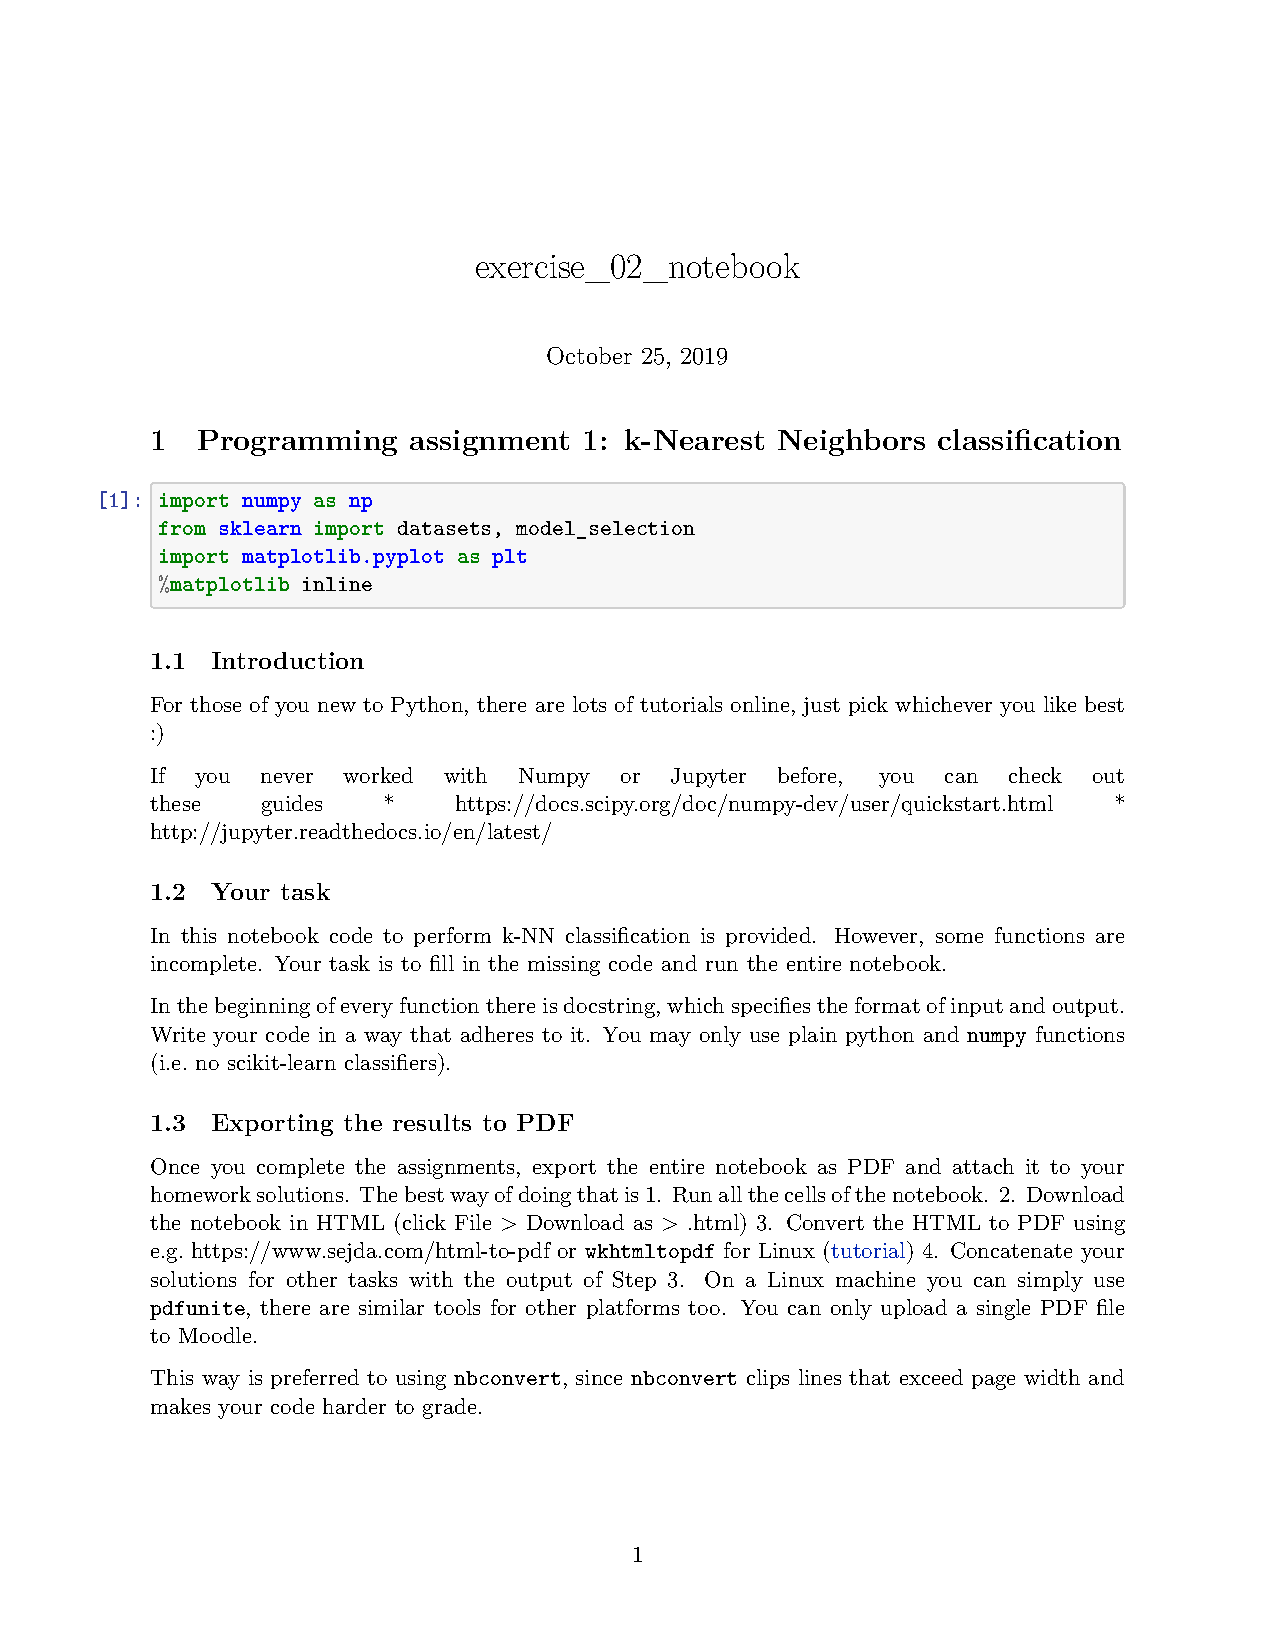
\includepdf[pages=-]{exercise_02_notebook.pdf}
%
%%%%%%%%%%%%%%%%%%%%%%%%%%%%%%%%%%%%%%%%%%%%%%%%%%%%%%%%%%%%%%%%%%%%%%%%%%%%%%%%
% !!! HOMEWORK ENDS HERE !!!
%%%%%%%%%%%%%%%%%%%%%%%%%%%%%%%%%%%%%%%%%%%%%%%%%%%%%%%%%%%%%%%%%%%%%%%%%%%%%%%%

%%%%%%%%%%%%%%%%%%%%%%%%%%%%%%%%%%%%%%%%%%%%%%%%%%%%%%%%%%%%%%%%%%%%%%%%%%%%%%%%
\newpage

\vspace*{-15.8mm}
\fontsize{19pt}{21pt}\selectfont

\vspace{25.3mm}
Appendix

\normalsize\selectfont
\vspace{13.2mm}
We confirm that the submitted solution is original work and was written by us without further assistance. Appropriate credit has been given where reference has been made to the work of others.

\vspace{18.1mm}
\rule[-3.7mm]{\linewidth}{0.5pt}
Munich, \today, Signature \PersonOne

\vspace{18.1mm}
\rule[-3.7mm]{\linewidth}{0.5pt}
Munich, \today, Signature \PersonTwo

\vspace{18.1mm}
\rule[-3.7mm]{\linewidth}{0.5pt}
Munich, \today, Signature \PersonThree
 % !!! DON'T TOUCH !!!
%%%%%%%%%%%%%%%%%%%%%%%%%%%%%%%%%%%%%%%%%%%%%%%%%%%%%%%%%%%%%%%%%%%%%%%%%%%%%%%%

\end{document}
